% title: Flattening and reconstructing a pytree
% description: Flattening separates a Review's comment and score from its structure and static source label. Unflattening reconstructs the Review.
\documentclass[tikz,border=5pt]{standalone}
\usetikzlibrary{arrows.meta,calc,shapes.geometric}
\definecolor{numeric}{HTML}{4477AA}
\definecolor{textual}{HTML}{AA4499}

\tikzset{
    box/.style={draw, line width=0.8pt, minimum height=0.8cm,
                minimum width=1.8cm, inner sep=6pt, align=center},
    ir/.style={box},
    flow/.style={-{Stealth[length=5pt]}, line width=0.9pt},
    feedback/.style={flow, dashed},
    note/.style={font=\small, align=center},
    choice/.style={diamond, draw, line width=0.8pt,
                   aspect=2, inner sep=2pt, align=center},
}

\newcommand{\irframe}[2]{
    \draw[line width=0.8pt] #1 rectangle #2;
}

\newcommand{\transformarrow}[4][above]{
    \draw[flow] (#2) -- node[#1=6pt,note] {#4} (#3);
}

\begin{document}
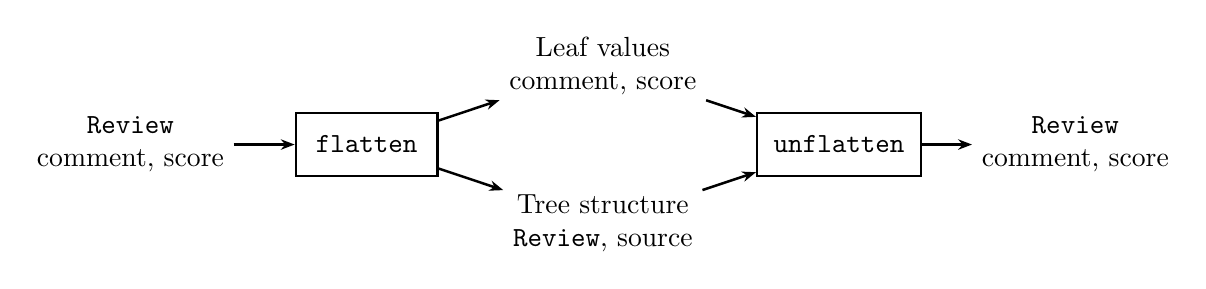
\begin{tikzpicture}

    \node[align=center] (state) at (0,0) {\texttt{Review}\\comment, score};
    \node[box] (flatten) at (3,0) {\texttt{flatten}};
    \node[align=center] (leaves) at (6,1) {Leaf values\\comment, score};
    \node[align=center] (spec) at (6,-1) {Tree structure\\\texttt{Review}, source};
    \node[box] (unflatten) at (9,0) {\texttt{unflatten}};
    \node[align=center] (result) at (12,0) {\texttt{Review}\\comment, score};
    \draw[flow] (state) -- (flatten);
    \draw[flow] (flatten) -- (leaves);
    \draw[flow] (flatten) -- (spec);
    \draw[flow] (leaves) -- (unflatten);
    \draw[flow] (spec) -- (unflatten);
    \draw[flow] (unflatten) -- (result);

\end{tikzpicture}
\end{document}
